\documentclass{article}

\usepackage{graphicx}
\usepackage{multirow}

\begin{document}

\begin{figure}

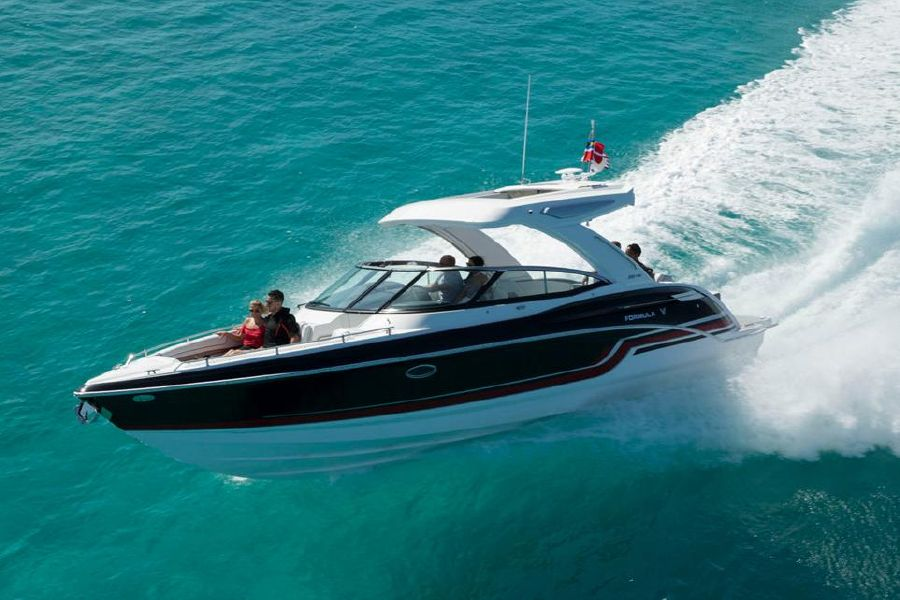
\includegraphics[width=\linewidth]{boat.jpg}

\caption{A boat.}

\label{fig:boatI}

\end{figure}

Figure \ref{fig:boatI}shows a boat\\

Table Example

\begin{table}[h!]
\begin{center}
\caption{Your first table.}
\label{tab:table1}
\begin{tabular}{l|c|r}

\textbf{Value 1} & \textbf{Value 2} & \textbf{Value 3} \\

$\alpha$ &$\beta$ & $\gamma$\\
\hline
1 & 1110.1 & a\\
2 & 10.1 & b\\
3 & 23.113231 & c\\
4 & 25.113231 & d\\ %

\end{tabular}
\end{center}

\end{table}

\begin{tabular}{ ||p{3cm}||p{3cm}||p{3cm}||  }
 \hline
 \multicolumn{3}{|c|}{Country List} \\
 \hline
 Country Name&Population&Literacy Rate\\
 \hline
 India   &  1.4B   &0.74\\
 America&   330M  & 0.99\\
 Australia &2.5M & 0.99\\
 Pakistan    &220M & 0.58\\
 Bangladesh& 160M  & 0.77\\
 \hline
\end{tabular}


\end{document}
